\documentclass[8pt]{extarticle}
\title{}
\author{Avinash Iyer}
\date{}
\usepackage[shortlabels]{enumitem}

%font setup
%
\usepackage{newpxtext,eulerpx}

%paper setup
\usepackage{geometry}
\geometry{letterpaper, portrait, margin=1in}
\usepackage{fancyhdr}

%symbols
\usepackage{amsmath}
\usepackage{mathtools}
\usepackage{amssymb}
\usepackage{hyperref}
\usepackage{gensymb}

\usepackage[T1]{fontenc}
\usepackage[utf8]{inputenc}

%chemistry stuff
\usepackage[version=4]{mhchem}
\usepackage{chemfig}

%plotting
\usepackage{pgfplots}
\usepackage{tikz}

%\usepackage{natbib}

%graphics stuff
\usepackage{graphicx}
\graphicspath{ {./images/} }

%code stuff
%when using minted, make sure to add the -shell-escape flag
%you can use lstlisting if you don't want to use minted
%\usepackage{minted}
%\usemintedstyle{pastie}
%\newminted[javacode]{java}{frame=lines,framesep=2mm,linenos=true,fontsize=\footnotesize,tabsize=3,autogobble,}
%\newminted[cppcode]{cpp}{frame=lines,framesep=2mm,linenos=true,fontsize=\footnotesize,tabsize=3,autogobble,}

\usepackage{listings}
\usepackage{color}
\definecolor{dkgreen}{rgb}{0,0.6,0}
\definecolor{gray}{rgb}{0.5,0.5,0.5}
\definecolor{mauve}{rgb}{0.58,0,0.82}

\lstset{frame=tb,
	language=Java,
	aboveskip=3mm,
	belowskip=3mm,
	showstringspaces=false,
	columns=flexible,
	basicstyle={\small\ttfamily},
	numbers=none,
	numberstyle=\tiny\color{gray},
	keywordstyle=\color{blue},
	commentstyle=\color{dkgreen},
	stringstyle=\color{mauve},
	breaklines=true,
	breakatwhitespace=true,
	tabsize=3
}
% text + color boxes
\usepackage{tcolorbox}
\tcbuselibrary{breakable}
\newtcolorbox{problem}[1]{colback = white, title = {#1}, breakable}
\newtcolorbox{solution}{colback = white, colframe = black!75!white, title = Solution, breakable}
%including PDFs
\usepackage{pdfpages}
\setlength{\parindent}{0pt}

\pagestyle{fancy}
\fancyhf{}
\rhead{Avinash Iyer}
\lhead{Problem Set 6}
\begin{document}
  \begin{problem}{Overstimulating the Economy}
    Suppose the economy today is producing output at its potential level and the inflation rate is equal to 2\%. What happens if policymakers try to stimulate the economy to keep output above potential for several years? How does your answer depend on the slope of the Phillips curve?
    \tcblower
    If policymakers try to stimulate the economy to keep output above potential for several years, then the economy will experience inflation --- if the Phillips curve is steep, then inflation will be far above 2\%, while if the Phillips curve is shallow, then inflation will be only modestly above 2\%.
  \end{problem}
  \begin{problem}{The Slope of the Phillips Curve}
    Draw a graph with a steep Phillips curve and a graph with a gently sloped Phillips curve.
    \begin{enumerate}[(a)]
      \item Explain how the two economies respond differently to a boom and to a slump.
      \item What are some factors that might influence the slope of the Phillips curve.
      \item Based on the graph below, do you think the slope of the Phillips curve has changed over time in the U.S. economy. Consider the United States in the 1970s versus today.
    \end{enumerate}
    \begin{center}
      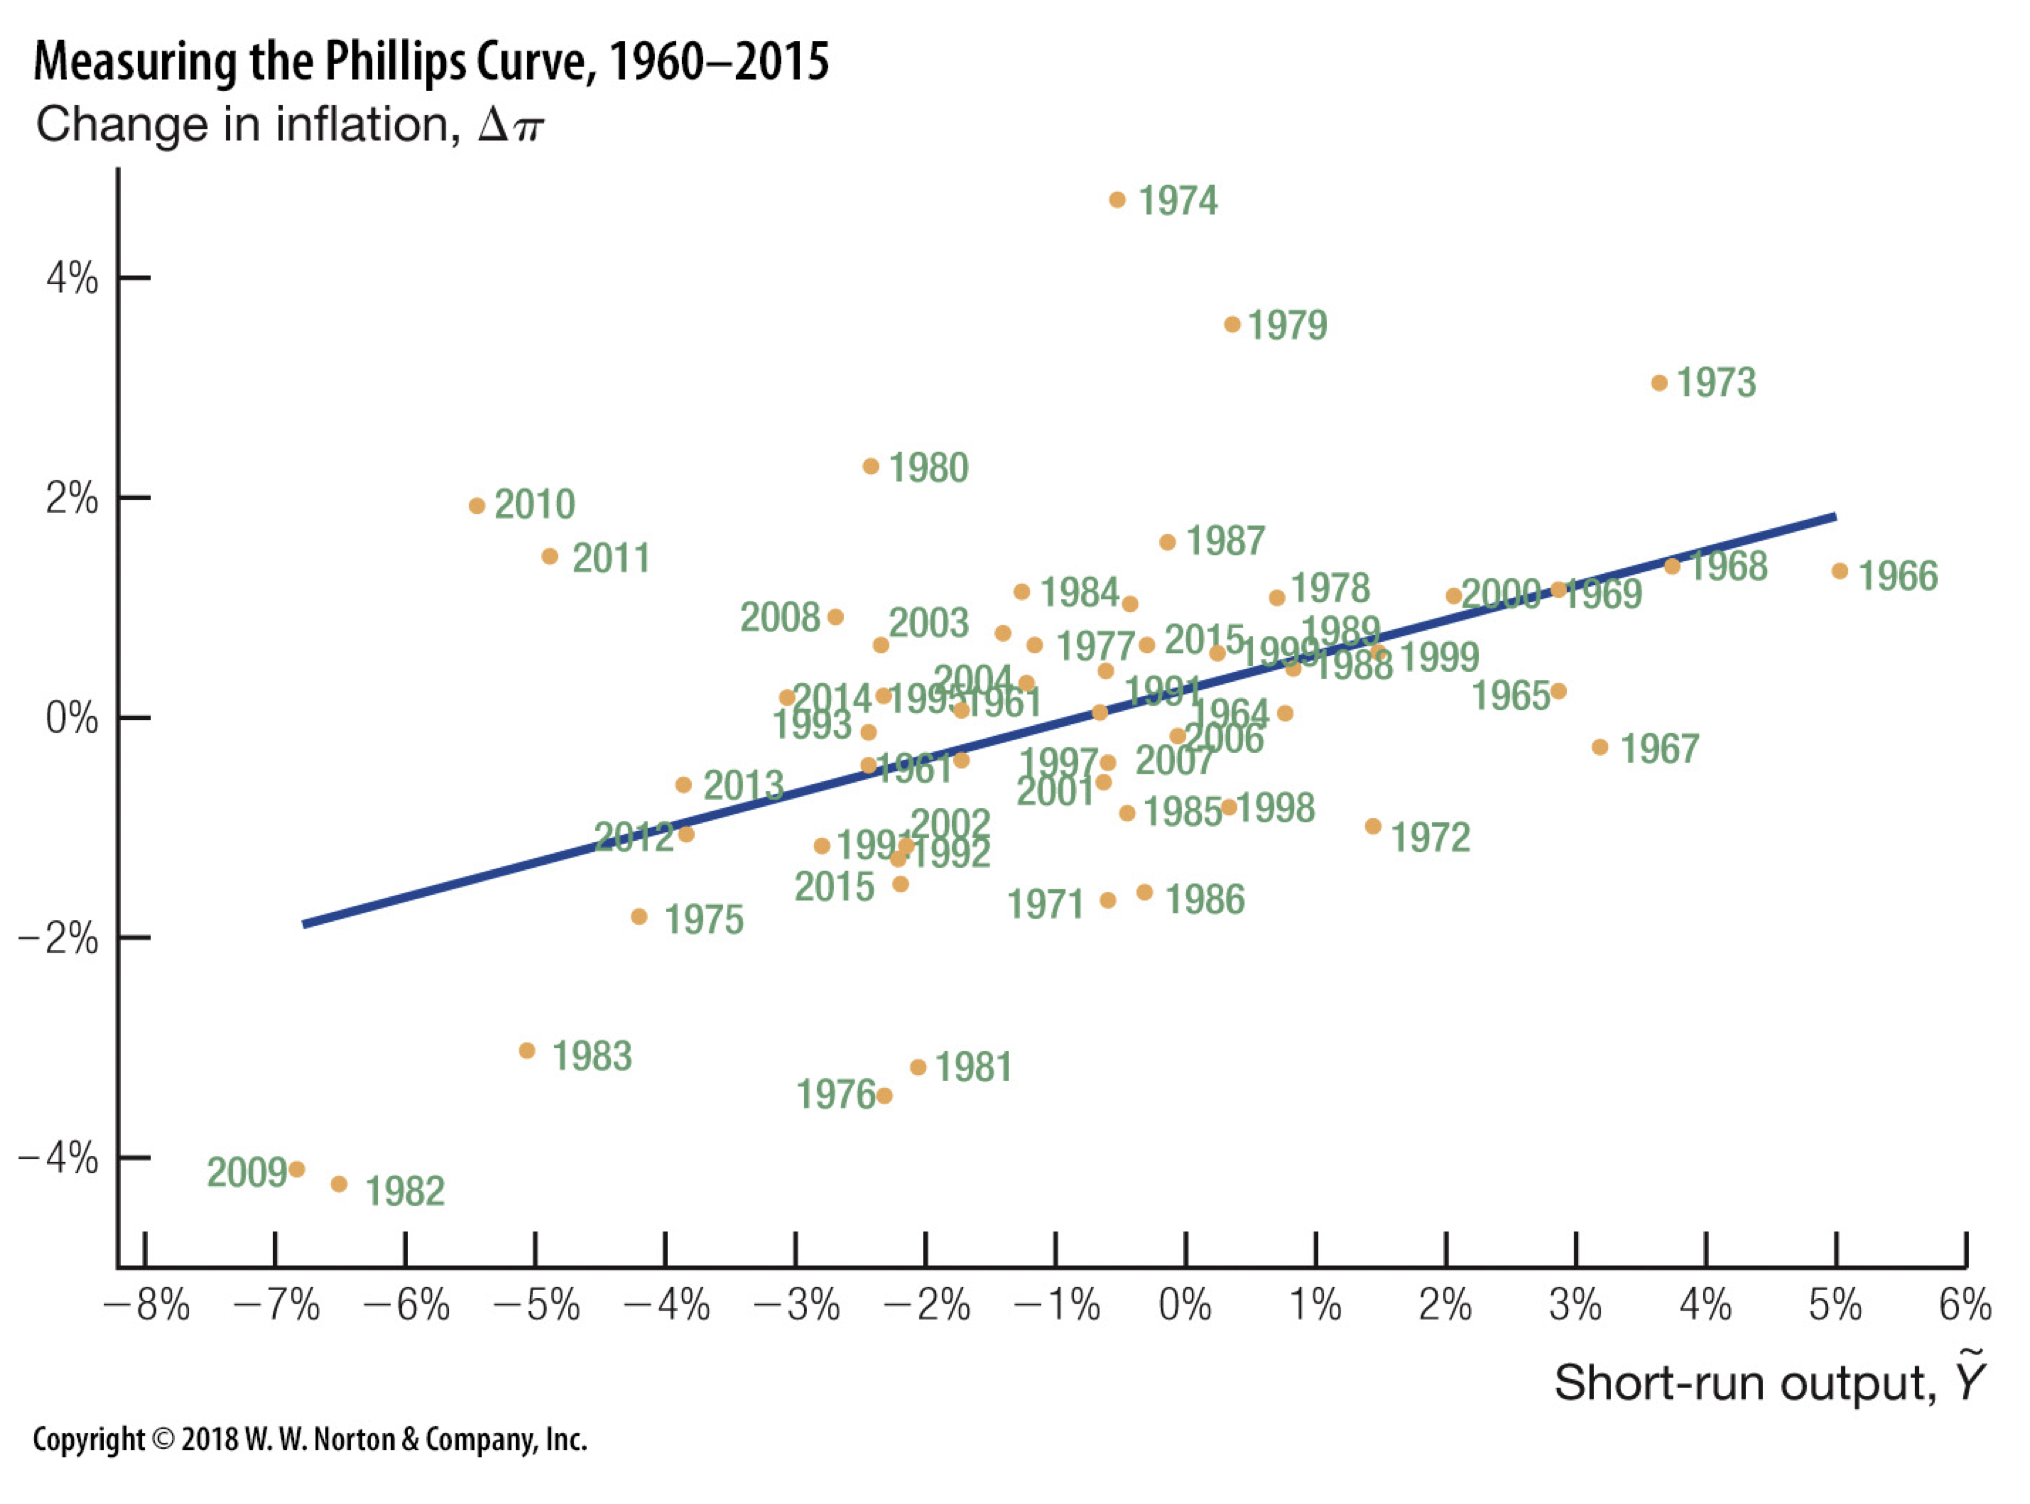
\includegraphics[width=10cm]{ps6_phillipscurveexample}
    \end{center}
    \tcblower
    \begin{center}
      \begin{tikzpicture}[scale = 0.5]
        \draw (-6,6) -- (-6,0) -- (0,0);
        \draw[thick] (-5,2) -- (-1,4);
        \node[anchor = west] at (0,0) {$\tilde{Y}$};
        \node [anchor = east] at (-6,6) {$\Delta \pi$};
        \draw[dashed] (-3,3) -- (-3,0);
        \draw[dashed] (-3,3) -- (-6,3);
      \end{tikzpicture}
      \qquad \qquad
      \qquad \qquad
      \begin{tikzpicture}[scale = 0.5]
        \draw (-6,6) -- (-6,0) -- (0,0);
        \draw[thick] (-4,1) -- (-2,5);
        \node[anchor = west] at (0,0) {$\tilde{Y}$};
        \node [anchor = east] at (-6,6) {$\Delta\pi$};
        \draw[dashed] (-3,3) -- (-3,0);
        \draw[dashed] (-3,3) -- (-6,3);
      \end{tikzpicture}
      \begin{tcolorbox}[colback = white, title = (a), breakable]
        The economy on the left, with a shallow Phillips curve, would see much less of a drastic change in inflation if output deviates from potential, while the economy on the right would see a substantial change to inflation if output slightly deviates from potential.
      \end{tcolorbox}
      \begin{tcolorbox}[colback = white, title = (b), breakable]
        The fundamentals of the economy such as employment rates, as well as policymakers' forward guidance, can possibly affect the slope of the Phillips curve.
      \end{tcolorbox}
      \begin{tcolorbox}[colback = white, title = (c), breakable]
        Looking at years such as the 1970s and 80s, we can see a very steep Phillips curve, but afterwards, with the advent of inflation targeting, the Phillips curve has flattened thanks to policymakers' forward guidance on expecting 2\% inflation.
      \end{tcolorbox}
    \end{center}
  \end{problem}
  \begin{problem}{A Productivity Boom}
    Suppose the economy exhibits a large, unexpected increase in productivity growth that causes potential output to rise substantially. Policymakers are (quite reasonably) slow to learn what has happened to potential output and incorrectly interpret the increase in output as a boom in which actual output exceeds potential. Suppose they adjust macroeconomic policy so that the mismeasured level of the output gap is zero.
    \begin{enumerate}[(a)]
      \item What happens to the true output gap?
      \item What happens to inflation over time?
    \end{enumerate}
    \tcblower
    \begin{enumerate}[(a)]
      \item The true output gap trends negative, since policymakers are expecting to adjust the positive output gap towards neutral, but instead are adjusting neutral downward.
      \item Since policymakers are creating a true negative output gap, they are creating negative inflation.
    \end{enumerate}
  \end{problem}
  \begin{problem}{Okun's Law}
    Assume that the economy has a natural rate of unemployment of 5\%.
    \begin{enumerate}
      \item Suppose that the output gap over the next four years is +1\%, 0\%, -1\%, and -2\%. According to Okun’s law, what unemployment rates would we expect to see in this economy?
      \item Consider another economy in which the unemployment rate over the next three years is 6\%, 7\%, and then 4\%. According to Okun’s Law, what is the output gap in this economy?
    \end{enumerate}
    \tcblower
    \begin{tcolorbox}[colback = white, title = (a), breakable]
      \begin{description}[font = \normalfont]
        \item[$\tilde{Y} = +1\%$:] $U = 4.5\%$
        \item[$\tilde{Y} = 0\%$:] $U = 5\%$
        \item[$\tilde{Y} = -1\%$:] $U = 5.5\%$
        \item[$\tilde{Y} = -2\%$:] $U = 6\%$
      \end{description}
    \end{tcolorbox}
    \begin{tcolorbox}[colback = white, title = (b), breakable]
      \begin{description}[font=\normalfont]
        \item[$U = 6\%$:] $\tilde{Y} = -2\%$
        \item[$U = 7\%$:] $\tilde{Y} = -4\%$
        \item[$U = 4\%$:] $\tilde{Y} = +2\%$
      \end{description}
    \end{tcolorbox}
  \end{problem}
  \begin{problem}{Analyzing Macroeconomic Events with the IS Curve}
    Consider the following changes in the macroeconomy. Show how to think about them using the IS curve, and explain how and why GDP is affected in the short run.
    \begin{enumerate}[(a)]
      \item The government offers a temporary investment tax credit.
      \item A booming economy in Europe this year leads to an unexpected increase in the demand by European consumers for American goods
      \item US Consumers develop an infatuation with all things made in New Zealand, and sharply increase their imports.
      \item A housing bubble bursts, so house prices fall by 20\% and new home sales drop sharply.
    \end{enumerate}
    \tcblower
    \begin{tcolorbox}[colback = white, title = (a), breakable]
      \begin{center}
        \begin{tikzpicture}[scale = 0.5]
          \draw (0,10) -- (0,0) -- (10,0);
          \node[anchor = west] at (10,0){$\tilde{Y}$};
          \node[anchor = east] at (0,10) {$R$};
          \draw[thick] (1,5) -- (5,1);
          \node[anchor = west] at (5,1) {IS$_1$};
          \draw[blue, thick] (1,7) -- (7,1);
          \node[anchor = west] at (7,1) {IS$_2$};
        \end{tikzpicture}
      \end{center}
      We can see here that the investment tax credit yields an increase in investment, and thus a positive output gap at any given interest rate.
    \end{tcolorbox}
    \begin{tcolorbox}[colback = white, title = (b), breakable]
      \begin{center}
        \begin{tikzpicture}[scale = 0.5]
          \draw (0,10) -- (0,0) -- (10,0);
          \node[anchor = west] at (10,0){$\tilde{Y}$};
          \node[anchor = east] at (0,10) {$R$};
          \draw[thick] (1,5) -- (5,1);
          \node[anchor = west] at (5,1) {IS$_1$};
          \draw[blue, thick] (1,7) -- (7,1);
          \node[anchor = west] at (7,1) {IS$_2$};
        \end{tikzpicture}
      \end{center}
      The increase in aggregate demand due to greater exports yields a positive output gap for any given rate of investment.
    \end{tcolorbox}
    \begin{tcolorbox}[colback = white, title = (c), breakable]
      \begin{center}
        \begin{tikzpicture}[scale = 0.5]
          \draw (0,10) -- (0,0) -- (10,0);
          \node[anchor = west] at (10,0){$\tilde{Y}$};
          \node[anchor = east] at (0,10) {$R$};
          \draw[thick] (1,5) -- (5,1);
          \node[anchor = west] at (5,1) {IS$_1=$ IS$_2$};
        \end{tikzpicture}
      \end{center}
      Since imports are counted in consumption and deleted in net exports, there is no change in the IS curve.
    \end{tcolorbox}
    \begin{tcolorbox}[colback = white, title = (d), breakable]
      \begin{center}
        \begin{tikzpicture}[scale = 0.5]
          \draw (0,10) -- (0,0) -- (10,0);
          \node[anchor = west] at (10,0){$\tilde{Y}$};
          \node[anchor = east] at (0,10) {$R$};
          \draw[thick] (1,5) -- (5,1);
          \node[anchor = west] at (5,1) {IS$_1$};
          \draw[blue, thick] (1,3) -- (3,1);
          \node[anchor = west] at (3,1) {IS$_2$};
        \end{tikzpicture}
      \end{center}
      There is a large drop in aggregate demand due to the fall in house prices, meaning that the IS curve shifts inward.
    \end{tcolorbox}
  \end{problem}
  \begin{problem}{Imports and the Multiplier}
    The amount of goods that the U.S. economy imports might depend on the current state of the economy as well as on potential GDP. For example, when the economy is booming, imports usually rise. Suppose the import equation is given as follows:
    \[
      \frac{IM_t}{\overline{Y}_t} = \overline{a}_{im} + \overline{n}\tilde{Y}
    \]
    \begin{enumerate}[(a)]
      \item Derive the IS curve for this new specification.
      \item What is the economic explanation for why $\overline{n}$ shows up in the denominator of the new IS curve?
    \end{enumerate}
    \tcblower
    \begin{tcolorbox}[colback = white, title = (a), breakable]
      \begin{align*}
        Y_t &= C_t + I_t + G_t + EX_t - IM_t \\
        \frac{Y_t}{\overline{Y}_t} &= \frac{C_t}{\overline{Y}_t} + \frac{I_t}{\overline{Y}_t} + \frac{G_t}{\overline{Y}_t} + \frac{EX_t}{\overline{Y}_t} - \frac{EX_t}{\overline{Y}_t} \\
        \frac{Y_t}{\overline{Y}_t} &= \overline{a}_c + \overline{a}_i - \overline{b}(R_t - \overline{r}) + \overline{a}_g + \overline{a}_{ex} - \overline{a}_{im} - \overline{n}\tilde{Y} \\
        \tilde{Y} + \overline{n}\tilde{Y}&= \left(\overline{a}_c + \overline{a}_i + \overline{a}_g + \overline{a}_{ex} - \overline{a}_{im}-1\right)- \overline{b}(R_t - \overline{r})  \\
        \tilde{Y} &= \frac{\overline{a} - \overline{b}(R_t - \overline{r})}{1+\overline{n}}
      \end{align*}
    \end{tcolorbox}
    \begin{tcolorbox}[colback = white, title = (b), breakable]
      If the share of imports rises, there should be a ``crowding out'' effect of domestic consumption, which is why the IS curve contains a $\overline{n}$ in the denominator.
    \end{tcolorbox}
  \end{problem}
  \begin{problem}{True/False}
    According to the Phillips curve, inflation rises when output is above its potential level because the higher level of output increases the amount of money that people want to hold, which leads the central bank to increase the money supply.
    \tcblower
    \textbf{False:} The higher level of output increases the amount of money that people want to \textit{spend}, which leads the central bank to increase the money supply.
  \end{problem}
  \begin{problem}{The Benefits of Price Stability}
    In his 2006 speech ``The Benefits of Price Stability,'' Ben Bernanke argues that price stability --- low and stable inflation --- fosters a stronger economy.
    \begin{quote}
        I will argue for what I believe has become the consensus view, that the mandated goals of price stability and maximum employment are almost entirely complementary. Central bankers, economists, and other knowledgeable observers around the world agree that price stability both contributes importantly to the economy's growth and employment prospects in the longer term and moderates the variability of output and employment in the short to medium term.
    \end{quote}
    Compile a list of the costs of high and variable inflation cited in the speech.
    \tcblower
    \begin{itemize}
      \item High and variable inflation can lead to costly bailouts and crises that taxpayers will have to foot the bill for.
      \item Price stability allows tax laws, accounting rules, wages, prices, etc. to be expressed in dollar amounts rather than forcing these fundamental parts of the economy to be indexed.
      \item High and variable inflation complicates long term economic planning for households and businesses.
      \item Dollar prices only provide proper signals of real value (as expected by price theory) when the price level is stable and predictable.
      \item High and variable inflation is a drag on economic growth.
      \item Stable prices lead to stable interest rates (Fisher effect).
    \end{itemize}
  \end{problem}
  \begin{problem}{FRED}
    The Federal Reserve Economic Database contains macroeconomic data series for the United States, with readily available graphs.
    \begin{enumerate}[(a)]
      \item Create a graph of real gross domestic product per capita starting in 1947 continuing until the present.
      \item Create a graph of real gross domestic product since January 1990.
      \item On the graph in part (b), add the line for real potential gross domestic product. What is the longest continuous period since 1990 in which actual GDP fell noticeably below potential?
      \item Create a graph of the output gap since 1990.
      \item Create a graph for another data series.
    \end{enumerate}
    \tcblower
    \begin{tcolorbox}[colback = white, title = (a), breakable]
      \begin{center}
        \begin{tikzpicture}
          \begin{axis}[
              title = {Real GDP Per Capita, dollars},
              xlabel = {Year},
              ylabel = {Real GDP Per Capita},
             y tick label style={/pgf/number format/.cd,%
          scaled y ticks = false,
          set thousands separator={},
          fixed}, xmin = 1947, xmax = 2023,
              x tick label style={/pgf/number format/.cd,%
          scaled y ticks = false,
          set thousands separator={},
          fixed},ymin = 10000, ymax = 70000,
              ytick = {10000,20000,30000,40000,50000,60000,70000},
            width=\textwidth,
            axis lines = left,height=\axisdefaultheight
            ]
            \addplot[color=blue] table[x index=0, y index=1]{images/ps6_rgdp_pc.dat};
          \end{axis}
        \end{tikzpicture}
      \end{center}
    \end{tcolorbox}
    \begin{tcolorbox}[colback = white, title = (b), breakable]
      \begin{center}
        \begin{tikzpicture}
          \begin{axis}[
              title = {Real GDP, Billions of dollars},
              xlabel = {Year},
              ylabel = {Real GDP},
             y tick label style={/pgf/number format/.cd,%
          scaled y ticks = false,
          set thousands separator={},
          fixed}, xmin = 1990, xmax = 2023,
              x tick label style={/pgf/number format/.cd,%
          scaled y ticks = false,
          set thousands separator={},
          fixed},ymin = 8000, ymax = 22000,
              ytick = {8000,10000,12000,14000,16000,18000,20000,22000},
            width=\textwidth,
            axis lines = left,height=\axisdefaultheight
            ]
            \addplot[color=blue] table[x index=0, y index=1]{images/ps6_rgdp_1990.dat};
          \end{axis}
        \end{tikzpicture}
      \end{center}
    \end{tcolorbox}
    \begin{tcolorbox}[colback = white, title = (c), breakable]
      \begin{center}
        \begin{tikzpicture}
          \begin{axis}[
              title = {Real GDP vs Potential, Billions of dollars},
              xlabel = {Year},
              ylabel = {Real GDP/Potential Real GDP},
             y tick label style={/pgf/number format/.cd,%
          scaled y ticks = false,
          set thousands separator={},
          fixed}, xmin = 1990, xmax = 2023,
              x tick label style={/pgf/number format/.cd,%
          scaled y ticks = false,
          set thousands separator={},
          fixed},ymin = 8000, ymax = 22000,
              ytick = {8000,10000,12000,14000,16000,18000,20000,22000},
            width=\textwidth,
            axis lines = left,height=\axisdefaultheight,
            legend pos = south east
            ]
            \addplot[color=blue] table[x index=0, y index=1]{images/ps6_rgdp_potential.dat};
            \addlegendentry{Real GDP}
            \addplot[color=red] table[x index=0, y index=2]{images/ps6_rgdp_potential.dat};
            \addlegendentry{Real Potential GDP}
          \end{axis}
        \end{tikzpicture}
      \end{center}
      The longest period where real GDP was below potential was the period between 2008 and 2019 following the Great Recession.
    \end{tcolorbox}
    \begin{tcolorbox}[colback = white, title = (d), breakable]
      \begin{center}
        \begin{tikzpicture}
          \begin{axis}[
              title = {Output Gap},
              xlabel = {Year},
              ylabel = {Output Gap},
             y tick label style={/pgf/number format/.cd,%
          scaled y ticks = false,
          set thousands separator={},
          fixed}, xmin = 1990, xmax = 2023,
              x tick label style={/pgf/number format/.cd,%
          scaled y ticks = false,
          set thousands separator={},
          fixed},ymin = -12.5, ymax = 2.5,
              ytick = {-12.5,-10,-7.5,-5,-2.5,0,2.5},
            width=\textwidth,
            axis lines = left,height=\axisdefaultheight
            ]
            \addplot[color=blue] table[x index=0, y index=1]{images/ps6_output_gap.dat};
            \draw[thin, gray](axis cs: 1990,0) -- (axis cs:2022.75,0);
          \end{axis}
        \end{tikzpicture}
      \end{center}
      The peak output decline during the Great Recession was a 5.7\% drop in output, while the peak output decline during the COVID-19 recession was a 11.6\% drop in output
    \end{tcolorbox}
    \begin{tcolorbox}[colback = white, title = (e), breakable]
      \begin{center}
        \begin{tikzpicture}
          \begin{axis}[
              title = {Producer Price Index, Wood},
              xlabel = {Year},
              ylabel = {Index (January 1982 = 100)},
             y tick label style={/pgf/number format/.cd,%
          scaled y ticks = false,
          set thousands separator={},
          fixed}, xmin = 1947, xmax = 2023,
              x tick label style={/pgf/number format/.cd,%
          scaled y ticks = false,
          set thousands separator={},
          fixed},ymin = 0, ymax = 500,
              ytick = {0,100,200,300,400,500},
            width=\textwidth,
            axis lines = left,height=\axisdefaultheight
            ]
            \addplot[color=blue] table[x index=0, y index=1]{images/ps6_ppi_wood.tsv};
          \end{axis}
        \end{tikzpicture}
      \end{center}
    \end{tcolorbox}
  \end{problem}
\end{document}
